\chapter{Parameter Estimation}



The cost function (see definition \ref{def:cost_function}) associates a numerical penalty to the Robot's action and thus the details of it determine the decisions made by the Robot. Under certain conditions, a cost function can be shown to exist~\citep{lavalle2006planning}, however, there is no systematic way of producing or deriving the cost function beyond applied logic. In general, the topic can be split into considering a continuous and discrete action space, $\mathbb{U}$. 	

\section{Continuous Action Space}
In case of a continuous action space, the cost function is typically picked from a set of standard choices.	

\begin{definition}[Quadratic Cost Function ($L_2$)]
	\label{def:quadratic_cost}
	The quadratic cost function (often referred to as $L_2$) is defined as
	\begin{equation}
		C(U(x,D_x,D_s),s) \equiv (U(x,D_x,D_s)-s)^2.
	\end{equation}
\end{definition}

\begin{theorem}[Mean Squared Error (MSE)]
	\label{theorem:MSE}
	Let $s\in \mathbb{R}$ a continuous scalar, then 
	\begin{equation}
		\begin{split}
			\mathbb{E}[C(U, S)|s,D_s,I] &= \mathbb{E}[(U-s)^2|s,D_s,I]\\ 
			&= \mathbb{E}[(U-\mathbb{E}[U])^2]+(s-\mathbb{E}[U])^2\\
			&=\text{Var}[U]+\text{Bias}[U]^2\\
		\end{split}
		\label{eq:MSE}
	\end{equation}
	where conditions have been suppressed in the second line (to fit to the page) and the bias of the estimator of $\hat{\vec{\theta}}$ is defined viz
	\begin{equation}
		\text{Bias}[U(x,D_x,D_s)]\equiv s-\mathbb{E}[U(x,D_x,D_s)|s,D_s,I].
	\end{equation}
	If $\mathbb{E}[C(U, S)|s,D_s,I]\xrightarrow[]{n\rightarrow\infty} 0$ then $C(U, S)$ is a weakly consistent estimate of $s$. There can be different consistent estimates that converge towards $s$ at different speeds. It is desirable for an estimate to be consistent and with small (quadratic) risk, meaning that both the bias and variance of the estimator should be small. In many cases, however, there is bias-variance which means that both cannot be minimized at the same time. 
\end{theorem}

\begin{corollary}[MLE is Approximately Minimax for \( L_2 \) Loss]
	\label{cor:MLE_minimax}
	Under certain regularity conditions, the Maximum Likelihood decision rule (MLE) \(U_{\text{MLE}}\) is approximately minimax for the \( L_2 \) loss function, meaning it approximately minimizes the maximum expected risk.
	
	\begin{proof}
		From theorem \ref{theorem:MSE}
		\begin{equation}
			\mathbb{E}[(U-s)^2|s,D_s,I] = \text{Var}[U]+\text{Bias}[U]^2.
		\end{equation}
		Under the regularity conditions where the MLE is unbiased and has asymptotically minimal variance, the bias term \(\text{Bias}(\hat{\theta}_{\text{MLE}}) = 0\) and the variance term \(\text{Var}(\hat{\theta}_{\text{MLE}})\) is minimized among a class of estimators. Thus, the expected \( L_2 \) loss for the MLE can be approximated by:
		\begin{equation}
			\mathbb{E}[(\hat{\theta}_{\text{MLE}} - \theta)^2] \approx \text{Var}(\hat{\theta}_{\text{MLE}}).
		\end{equation}
		
		To show the minimax property, consider the minimax risk defined as:
		\begin{equation}
			\inf_{\hat{\theta}} \sup_{\theta \in \Theta} \mathbb{E}[(\hat{\theta} - \theta)^2].
		\end{equation}
		
		Since the MLE asymptotically achieves the Cramér-Rao lower bound for variance, it approximately attains the infimum in the minimax criterion:
		\begin{equation}
			\sup_{\theta \in \Theta} \mathbb{E}[(\hat{\theta}_{\text{MLE}} - \theta)^2] \approx \inf_{\hat{\theta}} \sup_{\theta \in \Theta} \mathbb{E}[(\hat{\theta} - \theta)^2].
		\end{equation}
		
		Therefore, the MLE is approximately minimax under the \( L_2 \) loss function.
	\end{proof}
\end{corollary}


============== TO THIS POINT ========


\begin{example}
	One often encounter the trade-off between bias and variance in regression analysis. In regression analysis a model is trained on a set of training data and then tested on a set of test data. The training consists of estimating the relevant parameters for the model. There is a bias from selecting the model which is trained on the training data. This bias is increasingly smaller the more degrees of freedom there is in the model - meaning the bias decreases the better the model can fit the "wiggles" in the data. However, the better the model can fit the "wiggles" in the data, the more the model will vary when trained on different sets of training data, meaning the variance will be higher. You cannot have a model that fits every "wiggle" in the data perfectly \emph{and} never varies between training data sets. This is because there are random errors in data.
\end{example}

\begin{example}
	\emph{Consider $X_1,\dots, X_n\sim Ber(\vec{\theta})$. Determine the (quadratic) risk of three different estimators for the mean; the arithmetic sample mean, the number $0.5$ and the first data entry and $X_1$.}\newline
	
	\begin{itemize}
		\item For the arithmetic mean $\mathbb{E}[\hat{\vec{\theta}}]=\vec{\theta}$ and $Var[\hat{\vec{\theta}}]=\vec{\theta}(1-\vec{\theta})$, meaning that
		\begin{equation}
			\mathbb{E}[(\hat{\vec{\theta}}-\vec{\theta})^2]=\frac{\vec{\theta}(1-\vec{\theta})}{n}.
		\end{equation}
		
		\item For the number $0.5$ $Bias[\hat{\vec{\theta}}]=0.5-\vec{\theta}$ whereas $Var[\hat{\vec{\theta}}]=0$, so
		\begin{equation}
			\mathbb{E}[(\hat{\vec{\theta}}-\vec{\theta})^2]=(0.5-\vec{\theta})^2.
		\end{equation}
		
		\item For the first entry, $X_1$, $Bias[\hat{\vec{\theta}}]=0$ whereas $Var[\hat{\vec{\theta}}]=\vec{\theta}(1-\vec{\theta})$, so
		\begin{equation}
			\mathbb{E}[(\hat{\vec{\theta}}-\vec{\theta})^2]=\vec{\theta}(1-\vec{\theta}).
		\end{equation}
	\end{itemize}
	In conclusion it can be seen that the first entry is always a worse estimate for the population mean than the arithmetic sample mean. However, the number $0.5$ will actually be a better estimate of the population mean for a given range of $\vec{\theta}$.  
	\begin{figure}[H]
		\captionsetup{width=1\textwidth}
		\centering
		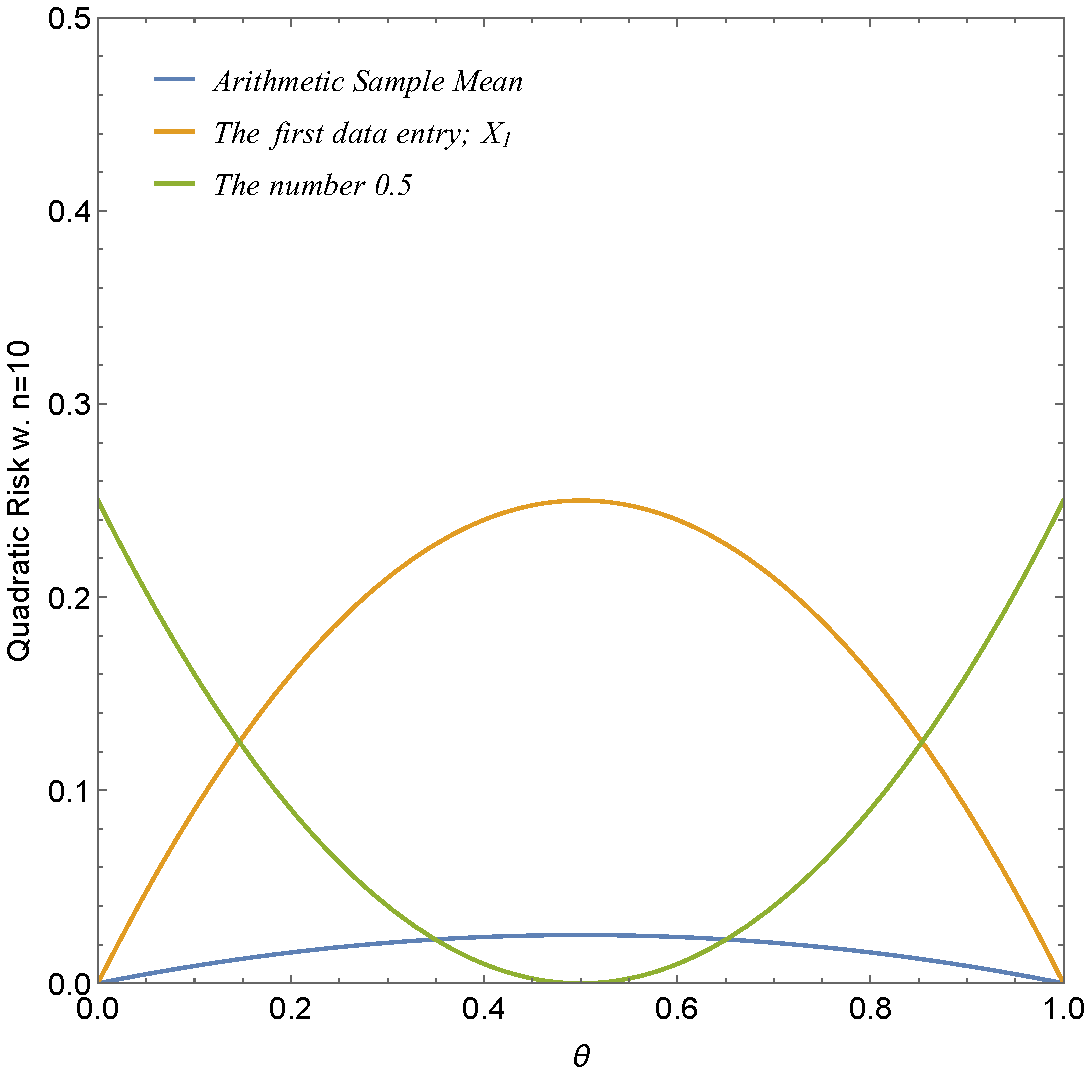
\includegraphics[width=0.4\textwidth]{figures/P1.pdf}
		\caption{}
		\label{fig:pen}
	\end{figure}
	
\end{example}


\begin{enumerate}
	\item The bias-variance decomposition is only relevant for frequentist statistics and Bayesian statistics does not struggle with this tradeoff. It relates to overfitting and underfitting. Bayesians do not fit in the same way as frequentists do. They do not determine a single set of parameters, rather they use a set of parameters due to integration. In that sense, they are protected against overfitting and underfitting and they do not struggle with hyperparameter finetuning as well.
	\item zero-one loss function leads to hypothesis testing.
	\item Can you derive the CI from a loss function?
	\item make example using decision rule k*x, from lecture\_1\_handout.
	\item admissibility for selecting frequentist decision rules. Also discuss dominated.
	\item is there a loss function that leads to maximum likelihood? How is ML related to the loss function and decision theory?
\end{enumerate}


=========================

Following section \ref{sec:framing_statistics}, statistics is framed as a game between a Robot and Nature in which each make decisions and the Robot is penalized for deviations from Natures actions via a cost function. The goal of the Robot is to minimize the expected cost associated with its decisions. To achieve this goal, the Robot utilizes its observations $x,D$ and background information $I$ to inform its decision-making process. Treating Natures decision $s\in \Omega_S$ as a fixed parameter, the conditional expected cost, can be written~\cite{murphy2023probabilistic}
\begin{equation}
	\label{eq:conditional_expected_cost2}
	\begin{split}
		\mathbb{E}[C(U,s)|s,D_s,I] &= \int d\tilde{D}_x  C(U(\tilde{D}_x,D_s),s) p(\tilde{D}_x|s,D_s,I)\\
	\end{split}
\end{equation}
where $D_s = \{s_1,s_2,\dots s_n\}$, $D_x = \{X_1 = x_1, X_2=x_2,\dots X_n=x_n\}$, $\tilde{D}_x = \{X=x,D_x\}$ and the Robot aims to find the decision rule which minimizes equation \eqref{eq:conditional_expected_cost2}. Because equation \eqref{eq:conditional_expected_cost2} depend on both the decision rule $U$ and $\{s,D_s\}$ (where $D_s$ is assumed known and $s$ unknown), no general solution exists without additional constraints to limit the solution space. 

\begin{definition}[Admissible Decision Rule]
	\label{def:admissible}
	A decision rule $U^*$ is said to be admissible if there exists no other decision rule $U'$ such that $\mathbb{E}[C(U', s) | s, D_s, I] \leq \mathbb{E}[C(U^*, s) | s, D_s, I]$ for all $s \in \Omega_S$.
\end{definition}

\begin{definition}[Dominating Decision Rule]
	\label{def:dominating}
	A decision rule $U'$ is said to dominate another decision rule $U^*$ if
	\begin{equation}
		\mathbb{E}[C(U', s) | s, D_s, I] \leq \mathbb{E}[C(U^*, s) | s, D_s, I]
	\end{equation}
	for all $s \in \Omega_S$ and $\exists s' \in \Omega_S$ such that
	\begin{equation}
		\mathbb{E}[C(U', s) | s', D_s, I] < \mathbb{E}[C(U^*, s) | s', D_s, I].
	\end{equation}
\end{definition}

\begin{definition}[Minimax Decision Rule]
	\label{def:minimax}
	A decision rule $U^*$ is said to be minimax if it minimize the maximum expected risk, meaning
	\begin{equation}
		U^* \equiv \inf_{U}\sup_{s\in \Omega_S}\mathbb{E}[C(U,s)|s,D_s,I].
	\end{equation}
\end{definition}





\begin{definition}[Maximum Likelihood Estimator (MLE) Decision Rule]
	\label{def:MLE}
	The Maximum Likelihood Estimator (MLE) decision rule $U_{\text{MLE}}$ is defined as the decision rule that maximizes the likelihood $p(D_s|\tilde{D}_x,s,I)$ given the data $\tilde{D}_x = D_x,X=x$ and past Nature decisions $D_s$
	\begin{equation}
		U_{\text{MLE}} \equiv \arg \max_{s} p(D_s|\tilde{D}_x,s,I).
	\end{equation}
\end{definition}






\begin{theorem}[Unbiasedness of the MLE]
	\label{thm:unbiased_mle}
	Under certain regularity conditions, the Maximum Likelihood Estimator $U_{\text{MLE}}$ is asymptotically unbiased, meaning
	\begin{equation}
		\mathbb{E}[U_{\text{MLE}}] = s \quad \text{for large sample sizes}.
	\end{equation}
\end{theorem}

\begin{proof}
	Given the data $\tilde{D}_x = D_x,X=x$ and past Nature decisions $D_s$, the MLE decision rule can be written
	\begin{equation}
		\begin{split}
			U_{\text{MLE}} &\equiv \arg \max_{s} p(D_s|\tilde{D}_x,s,I)\\
			&\equiv \arg \max_{s} \ln p(D_s|\tilde{D}_x,s,I)
		\end{split},
	\end{equation}
	where $p(D_s|\tilde{D}_x,s,I)$ is the likelihood and it has been used that $\ln$ is a monotonically increasing function for the second equality. For simplicity define the notation
	\begin{equation}
		l(s) \equiv \ln p(D_s|\tilde{D}_x,s,I).
	\end{equation}	
	Assuming $U_{\text{MLE}}\sim s$, $l(s)$ can be expanded around $U_{\text{MLE}}$ viz
	\begin{equation}
		l(s)\approx l(s)|_{s=U_{\text{MLE}}}+(s-U_{\text{MLE}})\frac{d}{ds}l(s)\bigg|_{s=U_{\text{MLE}}}.
	\end{equation}
	The MLE decision rule is defined by
	\begin{equation}
		\frac{d}{ds}l(s)\bigg|_{s=U_{\text{MLE}}} = 0,
	\end{equation}
	meaning
	\begin{equation}
		\frac{\frac{d}{ds}l(s)|_{s=U_{\text{MLE}}}}{\frac{d^2}{ds^2}l(s)|_{s=U_{\text{MLE}}}}\approx(s-U_{\text{MLE}})
	\end{equation}
	
	
	Under regularity conditions, the score function \( \ell'(\theta) = \frac{\partial}{\partial \theta} \log L(\theta; D_x, D_s) \) has an expected value of zero at the true parameter value \( \theta_0 \):
	\begin{equation}
		\mathbb{E}\left[\ell'(\theta)\bigg|_{\theta = \theta_0}\right] = 0.
	\end{equation}
	This implies that, on average, the log-likelihood is maximized at the true parameter value. 
	Assuming \(\hat{\theta}_{\text{MLE}}\) is close to \(\theta_0\), we can approximate:
	\[
	(\hat{\theta}_{\text{MLE}} - \theta_0) \approx - \frac{\ell'(\theta_0)}{\ell''(\theta_0)}.
	\]
	Now, taking the expectation:
	\[
	\mathbb{E}[\hat{\theta}_{\text{MLE}} - \theta_0] \approx - \mathbb{E}\left[\frac{\ell'(\theta_0)}{\ell''(\theta_0)}\right].
	\]
	Given that \(\mathbb{E}[\ell'(\theta_0)] = 0\), we get:
	\[
	\mathbb{E}[\hat{\theta}_{\text{MLE}} - \theta_0] = 0,
	\]
	which implies:
	\[
	\mathbb{E}[\hat{\theta}_{\text{MLE}}] = \theta_0.
	\]
\end{proof}

\begin{corollary}[MLE as Approximately Minimax]
	\label{cor:mle_minimax}
	Under certain regularity conditions, the MLE \( \hat{\theta}_{\text{MLE}} \) is approximately minimax with respect to the L2 loss function. Specifically,
	\begin{equation}
		\hat{\theta}_{\text{MLE}} \approx \inf_{U}\sup_{\theta} \mathbb{E}[(U - \theta)^2].
	\end{equation}
	This follows from the fact that the MLE is asymptotically unbiased and attains the Cramér-Rao lower bound, making it efficient and approximately minimax for large sample sizes.
\end{corollary}


\begin{theorem}[Unbiasedness of MLE under Regularity Conditions]
	\label{thm:MLE_unbiased}
	Under regularity conditions, the MLE \( U_{\text{MLE}} \) is an unbiased estimator of the true parameter \( s \), meaning
	\begin{equation}
		\mathbb{E}[U]= s.
	\end{equation}
	
	\begin{proof}
		Let $D_x = \{X_1 = x_1,X_2 =x_2,\dots X_n=x_n\}$ be data from a set of independent and identically distributed random variables from the measurable space $(\Omega,\mathcal{F})$, $s$ an unknown parameter and $p(X|s)$ a probability distribution for the generic random variable $X:\Omega\mapsto \Omega_X$. The log-likelihood can be written
		\begin{equation}
			\ln L(D_x|s) = \sum_{i=1}^n\ln p(X = x_i|s),
		\end{equation}
		meaning
		\begin{equation}
			\label{eq:lemur1}
			\begin{split}
				\mathbb{E}\bigg[\frac{\partial}{\partial s}\ln L(D_x|s)|s\bigg] &= \int  \frac{\partial}{\partial s} \sum_{i=1}^n\ln p(X_i = x_i|s) p(D_x|s) dD_x\\
				&= \int  \frac{\partial}{\partial s} \sum_{i=1}^n\ln p(X_i = x_i|s) p(X_i=x_i|s) dx_i\\
				&= \frac{\partial}{\partial s} \sum_{i=1}^n\int  p(X_i=x_i|s) dx_i\\
				&= 0.\\
			\end{split}
		\end{equation}
		Equation \eqref{eq:lemur1} means that the log-likelihood is maximized at $s$ and the maximum likelihood estimate does not systematically overestimate or underestimate $s$.
	\end{proof}
\end{theorem}
=================















\begin{definition}[Maximum Likelihood Estimator]
	\label{def:mle}
	The Maximum Likelihood Estimator (MLE) for a parameter \( \theta \) is the value \( \hat{\theta} \) that maximizes the likelihood function \( L(\theta; D_x, D_s) \), or equivalently, the log-likelihood function \( \ell(\theta) = \log L(\theta; D_x, D_s) \).
	\begin{equation}
		\hat{\theta}_{\text{MLE}} = \arg \max_{\theta} L(\theta; D_x, D_s).
	\end{equation}
\end{definition}

\begin{theorem}[Unbiasedness of the MLE]
	\label{thm:unbiased_mle}
	Under certain regularity conditions, the Maximum Likelihood Estimator \( \hat{\theta}_{\text{MLE}} \) is asymptotically unbiased, meaning:
	\begin{equation}
		\mathbb{E}[\hat{\theta}_{\text{MLE}}] \approx \theta_0 \quad \text{for large sample sizes}.
	\end{equation}
\end{theorem}

\begin{proof}
	
	
	
	Under the regularity conditions, the score function \( \ell'(\theta) = \frac{\partial}{\partial \theta} \log L(\theta; D_x, D_s) \) has an expected value of zero at the true parameter value \( \theta_0 \):
	\begin{equation}
		\mathbb{E}\left[\ell'(\theta)\bigg|_{\theta = \theta_0}\right] = 0.
	\end{equation}
	This implies that, on average, the log-likelihood is maximized at the true parameter value, and the MLE does not systematically overestimate or underestimate \( \theta \) as the sample size increases.
\end{proof}

\begin{corollary}[MLE as Approximately Minimax]
	\label{cor:mle_minimax}
	Under certain regularity conditions, the MLE \( \hat{\theta}_{\text{MLE}} \) is approximately minimax with respect to the L2 loss function. Specifically,
	\begin{equation}
		\hat{\theta}_{\text{MLE}} \approx \inf_{U}\sup_{\theta} \mathbb{E}[(U - \theta)^2].
	\end{equation}
	This follows from the fact that the MLE is asymptotically unbiased and attains the Cramér-Rao lower bound, making it efficient and approximately minimax for large sample sizes.
\end{corollary}






===========================


The performance of the maximum likelihood estimate is quantified by the \emph{Fischer information}. Define
\begin{equation}
	\ell(\vec{\theta})=log(L_1(X,\vec{\theta})), \quad \vec{\theta}\in\Theta\subset \mathbb{R}^d,
\end{equation}
where the subscript $1$ signifies that $X$ consist of only one random variable. The Fischer information of the statistical model is defined as
\begin{equation}
	I(\vec{\theta})=-\mathbb{E}[\vec{\nabla}^2\ell(\vec{\theta})].
\end{equation}
If this is large, the maximum likelihood estimate is good. Now let $\vec{\theta}^*\in \Theta$ (the true parameter) and assume
\begin{enumerate}
	\item The model is specified.
	\item $\forall \vec{\theta}\in \Theta$, the support of $\mathbb{P}_{\vec{\theta}}$ does not depend on $\vec{\theta}$.
	\item $\vec{\theta}^*$ is not on the boundary of $\Theta$.
	\item $I(\vec{\theta})$ is invertible in the neighborhood of $\vec{\theta}^*$.
	\item A few more technical conditions.
\end{enumerate}
Then, $\hat{\vec{\theta}}^{MLE}_n$ satisfies
\begin{equation}
	\hat{\vec{\theta}}_n^{MLE}\xrightarrow[]{n\rightarrow\infty}\vec{\theta}^* \quad (w.r.t. \, \mathbb{P}_{\vec{\theta}^*})\quad \wedge \quad \sqrt{n}(\hat{\vec{\theta}}_n^{MLE}-\vec{\theta}^*)\xrightarrow[]{n\rightarrow\infty}\mathcal{N}(0,I(\vec{\theta}^*)^{-1})\quad (w.r.t. \, \mathbb{P}_{\vec{\theta}^*}).
\end{equation}



\begin{definition}[Fisher Information]
	\label{def:fisher_information}
	The Fisher information is a way of measuring the amount of information about an unknown parameter a random variable contains. Let $s$ be an unknown parameter, $p(X|s)$ a probability distribution for the generic random variable $X:\Omega\mapsto \Omega_X$ and define $l(X|s)= \frac{\partial}{\partial s} \ln p(X|s)$. The Fisher information can then be written
	\begin{equation}
		\begin{split}
			I(s) &\equiv \mathbb{E} [l(X|s)^2|s]\\
			&= \text{Var}[l(X|s)|s]
		\end{split}
	\end{equation}
	where $p(X|s)$ is the probability density function of the observed data $D_x$ given the parameter $s$.
\end{definition}

\begin{proof}
	In general 
	\begin{equation}
		\mathbb{E} [l(X|s)^2|s] = \text{var}[l(X|s)|s]+\mathbb{E}[l(X|s)|s]^2
	\end{equation}
	however
	\begin{equation}
		\begin{split}
			\mathbb{E}[l(X|s)|s] &= \int  \frac{\partial}{\partial s} \ln p(X=x|s) p(X=x|s) dx\\
			&= \frac{\partial}{\partial s}\int  p(X=x|s) dx\\
			&= 0.\\
		\end{split}
	\end{equation}
\end{proof}


\begin{theorem}[Fisher information for sample]
	Let $X_1,X_2,\dots X_n$ be a set of independent and identically distributed random variables from the measurable space $(\Omega,\mathcal{F})$. The Fisher information in a sample is 
	\begin{equation}
		I(s) = nI_1(s),
	\end{equation}
	where $I_1(s)$ is the Fisher information of any one of the random variables.
\end{theorem}









===================
Given an observed sample $X_1,\dots, X_n$ and a statistical model $(E,(\mathbb{P}_{\vec{\theta}})_{\vec{\theta}\in \Theta})$, one wants to \emph{estimate} the parameter $\vec{\theta}$. The estimation is performed by a measurable\footnote{Rule of thumb: If you can calculate it, it is measurable.} function of the data (called a statistic) on the form
\begin{equation}
	\hat{\vec{\theta}}=\hat{\vec{\theta}}(X_1,\dots, X_n).
\end{equation}
Any function of the data can be an estimator, however, that estimator can be good or bad in relation to the parameter that is being estimated. An estimator is said to be (weakly) \emph{consistent} if when increasing the number of data points the estimate approach the true parameter in probability. That is
\begin{equation}
	\hat{\vec{\theta}}_n\xrightarrow[]{n\rightarrow\infty}\vec{\theta} \quad (w.r.t. \, \mathbb{P}_{\vec{\theta}}).
\end{equation}
Alternatively a consistent estimator, for which $\vec{\theta}\subseteq \mathbb{R}$, can be defined in terms of the quadratic ($l_2$) risk of $\hat{\vec{\theta}}$ 
\begin{equation}
	\begin{split}
		\mathbb{E}[(\hat{\vec{\theta}}-\vec{\theta})^2]&=\mathbb{E}[(\hat{\vec{\theta}}-\mathbb{E}[\hat{\vec{\theta}}]+\mathbb{E}[\hat{\vec{\theta}}]-\vec{\theta})^2]\\
		&=\mathbb{E}[(\hat{\vec{\theta}}-\mathbb{E}[\hat{\vec{\theta}}])^2]+2\mathbb{E}[(\hat{\vec{\theta}}-\mathbb{E}[\hat{\vec{\theta}}])(\mathbb{E}[\hat{\vec{\theta}}]-\vec{\theta})]+(\mathbb{E}[\hat{\vec{\theta}}]-\vec{\theta})^2\\
		&=\mathbb{E}[(\hat{\vec{\theta}}-\mathbb{E}[\hat{\vec{\theta}}])^2]+2{\mathbb{E}[(\hat{\vec{\theta}}-\mathbb{E}[\hat{\vec{\theta}}])]}(\mathbb{E}[\hat{\vec{\theta}}]-\vec{\theta})+(\mathbb{E}[\hat{\vec{\theta}}]-\vec{\theta})^2\\
		&=\mathbb{E}[(\hat{\vec{\theta}}-\mathbb{E}[\hat{\vec{\theta}}])^2]+(\mathbb{E}[\hat{\vec{\theta}}]-\vec{\theta})^2.\\
		&=Var[\hat{\vec{\theta}}]+(Bias[\hat{\vec{\theta}}])^2,\\
	\end{split}
\end{equation}
where the bias of the estimator of $\hat{\vec{\theta}}$ is defined viz
\begin{equation}
	Bias[\hat{\vec{\theta}}]\equiv \mathbb{E}[\hat{\vec{\theta}}]-\vec{\theta}.
\end{equation}
If $\mathbb{E}[[(\hat{\vec{\theta}}-\vec{\theta})^2]]\xrightarrow[]{n\rightarrow\infty} 0$ the $\hat{\vec{\theta}}$ is a weakly consistent estimator. There can be different consistent estimators that converge towards the true parameter at different speeds. It is desirable for an estimator to be consistent and with small (quadratic) risk, meaning that both the bias and variance of the estimator should be small. In many cases, however, there is bias-variance which means that both cannot be minimized at the same time. 

\begin{example}
	One often encounter the trade-off between bias and variance in regression analysis. In regression analysis a model is trained on a set of training data and then tested on a set of test data. The training consists of estimating the relevant parameters for the model. There is a bias from selecting the model which is trained on the training data. This bias is increasingly smaller the more degrees of freedom there is in the model - meaning the bias decreases the better the model can fit the "wiggles" in the data. However, the better the model can fit the "wiggles" in the data, the more the model will vary when trained on different sets of training data, meaning the variance will be higher. You cannot have a model that fits every "wiggle" in the data perfectly \emph{and} never varies between training data sets. This is because there are random errors in data.
\end{example}
\begin{example}
	\emph{Determine the (quadratic) risk of the arithmetic sample mean and variance weighted mean estimators of the population mean.}\newline
	
	\begin{itemize}
		\item The arithmetic sample mean estimator of the population mean is defined viz.
		\begin{equation}
			\begin{split}
				\hat{\mu}&=\bar{X}_n\\
				&=\frac{1}{n}\sum_{i=1}^{n}X_i.
			\end{split}
		\end{equation}
		The expectation value and variance 
		\begin{equation}
			\begin{split}
				&\mathbb{E}[\bar{X}_n]=\frac{1}{n}\sum_{i=1}^{n}\mathbb{E}[X_i]=\mu,\\
				&Var[\bar{X}_n]=\frac{1}{n^2}Var[\sum_{i=1}^{n}X_i]=\frac{1}{n^2}\sum_{i=1}^{n}Var[X_i],
			\end{split}
		\end{equation}
		where the possibility of $Var[X_i]\neq Var[X_j]$ has been retailed but $\mathbb{E}[X_i]=\mathbb{E}[X_j]=\mu$ has been assumed. This would e.g. be the case if each $X_i$ is measured with a separate apparatus in the experiment, or the a single apparatus that randomly vary in uncertainty between each single measurement. By assuming $\mathbb{E}[X_i]=\mathbb{E}[X_j]=\mu$ it is clear that the arithmetic mean has no bias. Therefore
		\begin{equation}
			\mathbb{E}[(\hat{\mu}-\mu)^2]=\frac{1}{n^2}\sum_{i=1}^{n}Var[X_i].
		\end{equation}
		
		\item The variance weighted sample mean estimator of the population mean is defined viz.
		\begin{equation}
			\begin{split}
				\hat{\mu}&=\bar{X'}_n\\
				&=\sum_{i=1}^{n}w'_iX_i,
			\end{split}
		\end{equation}
		where
		\begin{equation}
			w'_i\equiv \frac{w_i}{\sum_{j=1}^{n}w_j}.
		\end{equation}
		The expectation value and variance 
		\begin{equation}
			\begin{split}
				&\mathbb{E}[\bar{X'}_n]=\sum_{i=1}^{n}w'_i\mathbb{E}[X_i]=\mu,\\
				&Var[\bar{X'}_n]=Var[\sum_{i=1}^{n}w'_iX_i]=\sum_{i=1}^{n}(w'_i)^2Var[X_i],
			\end{split}
		\end{equation}
		with 
		\begin{equation}
			\frac{1}{n}\leq \sum_{i=1}^{n}(w'_i)^2\leq 1.
		\end{equation}
		Hence in this case
		\begin{equation}
			\mathbb{E}[(\hat{\mu}-\mu)^2]=\sum_{i=1}^{n}(w'_i)^2Var[X_i].
		\end{equation}
		Now take $w_i=\frac{1}{Var[X_i]}$. Hereby
		\begin{equation}
			\mathbb{E}[(\hat{\mu}-\mu)^2]=\frac{1}{\sum_{j=1}^{n}\frac{1}{Var[X_j]}}.
		\end{equation}
		
		In the case where $Var[X_i]=Var[x_j]$, the variance weighted mean is equal to the arithmetic mean. However, when $Var[X_i]\neq Var[x_j]$ the risk of the variance weighted mean is by definition smaller. Hence, whenever the data points have an associated uncertainty the variance weighted sample mean should be used to estimate the population mean.	
	\end{itemize}
\end{example}


\section{Confidence Interval}
Let $(E,(\mathbb{P}_{\vec{\theta}})_{\vec{\theta}\in \Theta})$ be a statistical model based on observations $X_1,\dots X_n$, and assume $\Theta\subseteq\mathbb{R}$. With $\alpha\in (0,1)$ a \emph{confidence interval} (C.I.) of level $1-\alpha$ for $\vec{\theta}$ is then any random (i.e. depending on $X$) interval, $\mathcal{I}$, whose boundaries do not depend on $\vec{\theta}$ and such that\footnote{$\mathcal{I}\ni \vec{\theta}$ means that $\mathcal{I}$ contains $\vec{\theta}$ and is meant to underline that the randomness is in $\mathcal{I}$.}
\begin{equation}
	\mathbb{P}_{\vec{\theta}}[\mathcal{I}\ni \vec{\theta}]\geq 1-\alpha, \quad \forall \vec{\theta}\in \Theta.
\end{equation} 
\begin{example}
	Let $X_1,\dots, X_n\sim Ber(p)$ with $n\gg 1$ for some unknown $p\in (0,1)$. Since $n\gg1 $ the PDF can be approximated by a standard normal distribution. Let $q_{\frac{\alpha}{2}}$ be the $(1-\frac{\alpha}{2})$-quantile of $\mathcal{N}(0,1)$ then
	\begin{equation}
		\begin{split}
			1-\alpha&=\lim\limits_{n\rightarrow \infty}\bigg[\mathbb{P}_p\bigg(\bigg|\frac{\bar{X}_n-p}{\sqrt{\frac{p(1-p)}{n}}}\bigg|\leq q_{\frac{\alpha}{2}}\bigg)\bigg]\\
			&=\lim\limits_{n\rightarrow \infty}\bigg[\mathbb{P}_p\bigg(\bar{X}_n-q_{\frac{\alpha}{2}}\sqrt{\frac{p(1-p)}{n}}\leq p \leq \bar{X}_n+q_{\frac{\alpha}{2}}\sqrt{\frac{p(1-p)}{n}}\bigg)\bigg],
		\end{split}
	\end{equation}
	and by extension	
	\begin{equation}
		\mathcal{I}=\bigg[\bar{X}_n-q_{\frac{\alpha}{2}}\sqrt{\frac{p(1-p)}{n}},\bar{X}_n+q_{\frac{\alpha}{2}}\sqrt{\frac{p(1-p)}{n}}\bigg].
	\end{equation}
	However, the C.I. should not depend on $p$, so let $p\rightarrow \hat{p}$ in the limits (Slutskys theorem)
	\begin{equation}
		\mathcal{I}=\bigg[\bar{X}_n-q_{\frac{\alpha}{2}}\sqrt{\frac{\hat{p}(1-\hat{p})}{n}},\bar{X}_n+q_{\frac{\alpha}{2}}\sqrt{\frac{\hat{p}(1-\hat{p})}{n}}\bigg],
	\end{equation}
	with 
	\begin{equation}
		\hat{p}=\bar{X}_n,
	\end{equation}
	since $p$ is the probability of a success in the experiment (success/failure experiment).
\end{example}

\section{Methods for Parameter Estimation}

\subsection{Maximum Likelihood Estimation}
Let $(E,(\mathbb{P}_{\vec{\theta}})_{\vec{\theta}\in \Theta})$ be a statistical model associated with a sample of i.i.d. random variables $X_1,\dots X_n$. Assume that there exists $\vec{\theta}^*\in\Theta$ such that $X_1\sim \mathbb{P}_{\vec{\theta}^*}:\vec{\theta}^*$ is the true parameter. Given $X_1,\dots X_n$ the goal is to find an estimator $\hat{\vec{\theta}}=\hat{\vec{\theta}}(X_1,\dots X_n)$ such that $\mathbb{P}_{\hat{\vec{\theta}}}$ is close to $\mathbb{P}_{\vec{\theta}^*}$ for the true parameter $\vec{\theta}^*$. This means
\begin{equation}
	|\mathbb{P}_{\hat{\vec{\theta}}}(A)-\mathbb{P}_{\vec{\theta}^*}(A)|=\text{small},\quad \forall A\subset E.
\end{equation}
The \emph{total variation distance} (TV) between two probability measures $\mathbb{P}_{\hat{\vec{\theta}}}$ and $\mathbb{P}_{\vec{\theta}'}$ is defined by
\begin{equation}
	TV(\mathbb{P}_{\hat{\vec{\theta}}},\mathbb{P}_{\vec{\theta}'})=\max_{A\subset E}|\mathbb{P}_{\hat{\vec{\theta}}}(A)-\mathbb{P}_{\vec{\theta}'}(A)|.
\end{equation}
If TV is small, then $\mathbb{P}_{\hat{\vec{\theta}}}\simeq \mathbb{P}_{\vec{\theta} '}$ $\forall >\subset E$. The TV obey 
\begin{equation}
	\begin{split}
		&TV(\mathbb{P}_{\vec{\theta}},\mathbb{P}_{\vec{\theta}'})=TV(\mathbb{P}_{\vec{\theta}'},\mathbb{P}_{\vec{\theta}})\quad \text{(Symmetric)},\\
		&TV(\mathbb{P}_{\vec{\theta}},\mathbb{P}_{\vec{\theta}'})\geq 0,\\
		&TV(\mathbb{P}_{\vec{\theta}},\mathbb{P}_{\vec{\theta}'})=0\,\text{if } \mathbb{P}_{\vec{\theta}}=\mathbb{P}_{\vec{\theta}'}\quad \text{(definite)},\\
		&TV(\mathbb{P}_{\vec{\theta}},\mathbb{P}_{\vec{\theta}'})\leq TV(\mathbb{P}_{\vec{\theta}''},\mathbb{P}_{\vec{\theta}})+TV(\mathbb{P}_{\vec{\theta}''},\mathbb{P}_{\vec{\theta}'})\quad \text{(Triangle inequality)}.\\
	\end{split}
\end{equation}
These identities imply that the total variation is a distance between probability distributions. Graphically $2TV$ is the area of two distributions that does not overlap. 
\begin{example}
	If $TV(\mathbb{P}_{\hat{\vec{\theta}}},\mathbb{P}_{\vec{\theta}'})\leq k$ then
	\begin{equation}
		\mathbb{P}_{\hat{\vec{\theta}}}(A)\in [\mathbb{P}_{\vec{\theta}'}(A)\pm k], \quad \forall A\subset E.
	\end{equation}
\end{example}
In the case of discrete and continuous random variables TV takes the form
\begin{equation}
	\begin{split}
		&TV(\mathbb{P}_{\vec{\theta}},\mathbb{P}_{\vec{\theta'}})=\frac{1}{2}\sum_{x_i\in E}|f_{\vec{\theta}}(x_i)-f_{\vec{\theta'}}(x_i)|\quad \text{For a discrete random variables},\\
		&TV(\mathbb{P}_{\vec{\theta}},\mathbb{P}_{\vec{\theta}'})=\frac{1}{2}\int_E|f_{\vec{\theta}}(x)-f_{\vec{\theta}'}(x)|\quad \text{For a continuous random variables}.
	\end{split}
\end{equation}
Ideally an estimator $\widehat{TV}(\mathbb{P}_{\hat{\vec{\theta}}},\mathbb{P}_{\vec{\theta}^*})$ for all $\vec{\theta}\in \Theta$ should now be constructed such that one could find $\hat{\vec{\theta}}$ that minimize the function $\vec{\theta}\mapsto \widehat{TV}(\mathbb{P}_{\hat{\vec{\theta}}},\mathbb{P}_{\vec{\theta}^*})$. However, there is no simple way of estimating $TV$, so a different, somewhat equivalent, measure (of which there are many) is considered; the Kullback-Leibler (KL) divergence. The KL divergence  between two probability measures $\mathbb{P}_{\vec{\theta}}$ and $\mathbb{P}_{\vec{\theta}'}$ is defined by
\begin{equation}
	KL(\mathbb{P}_{\vec{\theta}},\mathbb{P}_{\vec{\theta}'})=\begin{cases}
		\sum_{x_i\in E}f_{\vec{\theta}}(x_i)log\bigg(\frac{f_{\vec{\theta}}(x_i)}{f_{\vec{\theta'}}(x_i)}\bigg) \quad \text{If $E$ is discrete}\\
		\int_Edx f_{\vec{\theta}}(x)log\bigg(\frac{f_{\vec{\theta}}(x)}{f_{\vec{\theta'}}(x)}\bigg) \quad \text{If $E$ is continuous}\\
	\end{cases},
\end{equation}
where $log$ has an unspecified base. The KL divergence obey
\begin{equation}
	\begin{split}
		&TV(\mathbb{P}_{\vec{\theta}},\mathbb{P}_{\vec{\theta}'})\neq TV(\mathbb{P}_{\vec{\theta}'},\mathbb{P}_{\vec{\theta}})\quad \text{(in general)},\\
		&TV(\mathbb{P}_{\vec{\theta}},\mathbb{P}_{\vec{\theta}'})\geq 0,\\
		&TV(\mathbb{P}_{\vec{\theta}},\mathbb{P}_{\vec{\theta}'})=0\,\text{if } \mathbb{P}_{\vec{\theta}}=\mathbb{P}_{\vec{\theta}'}\quad \text{(definite)} ,\\
		&TV(\mathbb{P}_{\vec{\theta}},\mathbb{P}_{\vec{\theta}'})\nleq  TV(\mathbb{P}_{\vec{\theta}''},\mathbb{P}_{\vec{\theta}})+TV(\mathbb{P}_{\vec{\theta}''},\mathbb{P}_{\vec{\theta}'})\quad \text{(in general)}.\\
	\end{split}
\end{equation}
From these identities it is clear that the KL divergence is actually not a distance but a divergence. The KL divergence can be written in terms of the expectation value
\begin{equation}
	\begin{split}
		KL(\mathbb{P}_{\vec{\theta}^*},\mathbb{P}_{\vec{\theta}})&=\mathbb{E}_{\vec{\theta}^*}\bigg[log\bigg(\frac{f_{\vec{\theta}^*}(X)}{f_{\vec{\theta}}(X)}\bigg)\bigg]\\
		&=\mathbb{E}_{\vec{\theta}^*}[log(f_{\vec{\theta}^*}(X))]-\mathbb{E}_{\vec{\theta}^*}[log(f_{\vec{\theta}}(X))].
	\end{split}
\end{equation}
So, the function $\vec{\theta}\mapsto KL(\mathbb{P}_{\vec{\theta}^*},\mathbb{P}_{\vec{\theta}})$ is on the form $const-\mathbb{E}_{\vec{\theta}^*}[log(f_{\vec{\theta}}(X))]$. This can be estimated 
\begin{equation}
	\widehat{KL}(\mathbb{P}_{\vec{\theta}^*},\mathbb{P}_{\vec{\theta}})=const-\frac{1}{n}\sum_{i=1}^nlog(f_{\vec{\theta}}(X_i)).
\end{equation}
This is a candidate estimator for $KL$. Minimizing $\widehat{KL}$ will result in $\vec{\theta}\simeq \vec{\theta}^*$, so consider
\begin{equation}
	\begin{split}
		\argmin_{\vec{\theta}}(\widehat{KL}(\mathbb{P}_{\vec{\theta}^*},\mathbb{P}_{\vec{\theta}}))&=\argmin_{\vec{\theta}}\bigg(const-\frac{1}{n}\sum_{i=1}^nlog(f_{\vec{\theta}}(X_i))\bigg)\\
		&=\argmin_{\vec{\theta}}\bigg(-\frac{1}{n}\sum_{i=1}^nlog(f_{\vec{\theta}}(X_i))\bigg)\\
		&=\argmax_{\vec{\theta}}\bigg(\frac{1}{n}\sum_{i=1}^nlog(f_{\vec{\theta}}(X_i))\bigg)\\
		&=\argmax_{\vec{\theta}}\bigg(\sum_{i=1}^nlog(f_{\vec{\theta}}(X_i))\bigg)\\
		&=\argmax_{\vec{\theta}}\bigg(log\bigg(\prod_{i=1}^nf_{\vec{\theta}}(X_i)\bigg)\bigg)\\
	\end{split}
\end{equation}
where it has been used that the additive constant and constant rescaling factors does not change the location of the minimum or maximum. Since $log(f)$ is an increasing function, maximizing $log(f)$ is equivalent to maximizing $f$. Therefore
\begin{equation}
	\begin{split}
		\argmin_{\vec{\theta}}(\widehat{KL}(\mathbb{P}_{\vec{\theta}^*},\mathbb{P}_{\vec{\theta}}))\Leftrightarrow \argmax_{\vec{\theta}}\bigg(\underbrace{\prod_{i=1}^nf_{\vec{\theta}}(X_i)}_{\equiv likelihood}\bigg).\\
	\end{split}
\end{equation}
The likelihood is defined viz.
\begin{equation}
	L(\vec{\theta}|X_1,\dots,X_n)\equiv\prod_{i=1}^nf_{\vec{\theta}}(X_i).
	\label{ll}
\end{equation}
$L(\vec{\theta})$ is the joint density of the vector $(X_1,\dots, X_n)$. The likelihood is a concave function, meaning that if it has a local maximum it must also be the global maximum. The formal definition of the maximum likelihood estimator is as follows; let $X_1,\dots X_n$ be an i.i.d. sample associated with a statistical model $(E,(\mathbb{P}_{\vec{\theta}})_{\vec{\theta}\in \Theta})$ and let $L$ be the corresponding likelihood. The maximum likelihood estimator of $\vec{\theta}$ is then defined as
\begin{equation}
	\begin{split}
		\hat{\vec{\theta}}^{MLE}_n&\equiv \argmax_{\vec{\theta}\in \Theta}\bigg(L(X_1,\dots, X_n,\vec{\theta})\bigg)\\
		&= \argmax_{\vec{\theta}\in \Theta}\bigg(log(L(X_1,\dots, X_n,\vec{\theta}))\bigg)
	\end{split}
\end{equation}
provided it exists. The performance of the maximum likelihood estimate is quantified by the \emph{Fischer information}. Define
\begin{equation}
	\ell(\vec{\theta})=log(L_1(X,\vec{\theta})), \quad \vec{\theta}\in\Theta\subset \mathbb{R}^d,
\end{equation}
where the subscript $1$ signifies that $X$ consist of only one random variable. The Fischer information of the statistical model is defined as
\begin{equation}
	I(\vec{\theta})=-\mathbb{E}[\vec{\nabla}^2\ell(\vec{\theta})].
\end{equation}
If this is large, the maximum likelihood estimate is good. Now let $\vec{\theta}^*\in \Theta$ (the true parameter) and assume
\begin{enumerate}
	\item The model is specified.
	\item $\forall \vec{\theta}\in \Theta$, the support of $\mathbb{P}_{\vec{\theta}}$ does not depend on $\vec{\theta}$.
	\item $\vec{\theta}^*$ is not on the boundary of $\Theta$.
	\item $I(\vec{\theta})$ is invertible in the neighborhood of $\vec{\theta}^*$.
	\item A few more technical conditions.
\end{enumerate}
Then, $\hat{\vec{\theta}}^{MLE}_n$ satisfies
\begin{equation}
	\hat{\vec{\theta}}_n^{MLE}\xrightarrow[]{n\rightarrow\infty}\vec{\theta}^* \quad (w.r.t. \, \mathbb{P}_{\vec{\theta}^*})\quad \wedge \quad \sqrt{n}(\hat{\vec{\theta}}_n^{MLE}-\vec{\theta}^*)\xrightarrow[]{n\rightarrow\infty}\mathcal{N}(0,I(\vec{\theta}^*)^{-1})\quad (w.r.t. \, \mathbb{P}_{\vec{\theta}^*}).
\end{equation}

\begin{example}
	\emph{Determine the maximum likelihood estimate of $p$ for the model $(\{0,1\},\{Ber(p)\}_{p\in(0,1)})$.}\newline
	
	\noindent In this case
	\begin{equation}
		\begin{split}
			L(p)=\prod_{i=1}^np^{x_i}(1-p^{x_i}).
		\end{split}
	\end{equation}
	Considering the form of the likelihood function it is expedient to maximize the logarithm of the likelihood, such that
	\begin{equation}
		\begin{split}
			argmax_p\bigg(log(L(p))\bigg)&= argmax_p\bigg(log\bigg(\prod_{i=1}^np^{x_i}(1-p^{x_i})\bigg)\bigg)\\
			&= argmax_{p}\bigg(\bigg(\sum_{i=1}^nx_i\bigg)log(p)+\bigg(n-sum_{i=1}^nx_i\bigg)log(1-p)\bigg).
		\end{split}
	\end{equation}
	Now 
	\begin{equation}
		\frac{dlog(L(p))}{dp}=\frac{1}{log(base)}\bigg[\frac{\sum_{i=1}^nx_i}{p}-\frac{n-\sum_{i=1}^nx_i}{1-p}\bigg].
	\end{equation}
	Requiring the derivative to vanish means the maximum likelihood estimate of $p$ is given by
	\begin{equation}
		\hat{p}=\frac{1}{n}\sum_{i=1}^nx_i.
	\end{equation}
\end{example}
\begin{example}
	\emph{Determine the maximum likelihood estimate of $\lambda$ for the model $([0,\infty),\{Exp(\lambda)\}_{\lambda>0})$.}\newline
	
	\noindent In this case
	\begin{equation}
		\begin{split}
			L(\lambda)=\prod_{i=1}^n\lambda e^{-\lambda x_i}.
		\end{split}
	\end{equation}
	Again maximize the logarithm of the likelihood function
	\begin{equation}
		\frac{dlog(L(\lambda))}{d\lambda}=\frac{n}{\lambda}-\sum_{i=1}^nx_i
	\end{equation}
	Requiring the derivative to vanish means the maximum likelihood estimate of $\lambda$ is given by
	\begin{equation}
		\hat{\lambda}=\frac{1}{\frac{1}{n}\sum_{i=1}^nx_i}.
	\end{equation}
\end{example}

\subsection{The Method of Least Squares}
The method of least squares (LS) is the standard approach to regression analysis in which a statistic, $g$, describes a measured, quantitative response, $Y$. That is
\begin{equation}
	Y=g(X_1\dots X_n)+\varepsilon,
\end{equation}  
where $\varepsilon$ is an error-term - often it is assumed that $\varepsilon\sim\mathcal{N}(0,\sigma^2)$. In this equation $g(X_1\dots X_n)$ represents the systematic variations in $Y$ and $\varepsilon$ represent the random. However, in the case where unaccounted systematic measurement uncertainties are present in $Y$, and $g$ is known, $\varepsilon$ can contain systematic effects as well. The measured response is estimated by estimating $f$
\begin{equation}
	\hat{Y}=\hat{g}(X_1\dots X_n,\vec{\theta}).
\end{equation}
In the method of least squares $\hat{\vec{\theta}}$ is determined by minimizing the sum of squared residuals. 

\subsection{Independent $y_i$ and $x_i$} In the case where the measurements, $y_i$ and $x_i$, are independent (no systematic uncertainties occur in $\delta y_i$ and $\delta x_i$)
\begin{equation}
	S(\vec{\theta})=\sum_{i=1}^n\bigg[\bigg(\frac{y_i-\hat{g}(\hat{x}_i,\vec{\theta})}{\delta y_i}\bigg)^2+\bigg(\frac{x_i-\hat{x}_i}{\delta x_i}\bigg)^2\bigg],
	\label{eq6}
\end{equation}
where $\delta y_i$ and $\delta x_i$ are the uncertainties (standard deviations) of the individual measured data points and $\hat{x}$ is the (unknown\footnote{There is by definition no function that estimates the independent variable.}) estimate of the independent variable. $\hat{\vec{\theta}}$ is estimated via the least squares method viz
\begin{equation}
	\hat{\vec{ \theta}}_n^{LS}=\argmin_{\vec{\theta},\hat{x}}(S).
\end{equation}
The minimization can be be carried out via numerical iteration. However, the job can be simplified by carrying out the minimization over $\hat{x}$ analytically. Consider
\begin{equation}
	\begin{split}
		\frac{\partial S}{\partial \hat{x}_i}&=-2\frac{y_i-\hat{g}(\hat{x}_i,\vec{\theta})}{\delta y_i^2}\frac{\partial \hat{g}(\hat{x}_i,\vec{\theta})}{\partial \hat{x}_i}-2\frac{x_i-\hat{x}_i}{\delta x_i^2}\\
		&=0
	\end{split}
	\label{eq3}
\end{equation}
Now, let
\begin{equation}
	\hat{g}(x_i,\vec{\theta})=\hat{g}(\hat{x}_i,\vec{\theta})+(x_i-\hat{x}_i)\frac{\partial \hat{g}(x_i,\vec{\theta})}{\partial x_i}\bigg|_{x_i=\hat{x}_i}+\mathcal{O}(\partial^2\hat{g}).
	\label{eq4}
\end{equation}
Using equation \eqref{eq4} in \eqref{eq3}
\begin{equation}
	\begin{split}
		-\frac{y_i-[\hat{g}(x_i,\vec{\theta})-(x_i-\hat{x}_i)\frac{\partial \hat{g}(x_i,\vec{\theta})}{\partial x_i}\bigg|_{x_i=\hat{x}_i}]}{\delta y_i^2}\frac{\partial \hat{g}(\hat{x}_i,\vec{\theta})}{\partial \hat{x}_i}-\frac{x_i-\hat{x}_i}{\delta x_i^2}+\mathcal{O}(\partial^2\hat{g})=0.
	\end{split}
\end{equation}
Now, define $\hat{g'}\equiv \frac{\partial \hat{g}(x_i,\vec{\theta})}{\partial x_i}\bigg|_{x_i=\hat{x}_i}=\frac{\partial \hat{g}(\hat{x}_i,\vec{\theta})}{\partial \hat{x}_i}$. Hereby
\begin{equation}
	\begin{split}
		\hat{x}_i=x_i+\frac{\delta x_i^2}{\delta_i^2}(y_i-\hat{g}(x_i,\vec{\theta}))+\mathcal{O}(\partial^2\hat{g}),
	\end{split}
	\label{eq5}
\end{equation}
where
\begin{equation}
	\delta_i^2=\delta y_i^2+\delta x_i^2\hat{g'}^2.
\end{equation}
Using equation \eqref{eq5} and \eqref{eq4} in equation \eqref{eq6}
\begin{equation}
	S(\vec{\theta})\simeq\sum_{i=1}^n\bigg(\frac{y_i-\hat{g}(x_i,\vec{\theta})}{\delta_i}\bigg)^2.
	\label{eq7}
\end{equation}
Often the uncertainty of the independent variable can be neglected. In this case $\delta x_i\simeq 0$ and equation \eqref{eq7} becomes
\begin{equation}
	S(\vec{\theta})=\sum_{i=1}^n\bigg(\frac{y_i-\hat{g}(x_i,\vec{\theta})}{\delta y_i}\bigg)^2,
	\label{eq8}
\end{equation}
which is the famous equation of least squares. Least squares estimates for the parameters can now be obtained from
\begin{equation}
	\hat{\vec{ \theta}}_n^{LS}=\argmin_{\vec{\theta}\in \Theta}(S).
\end{equation}
In the case where $\delta x_i\neq 0$ equation \eqref{eq7} in its entirely must be applied. In doing so it should be noted that $\hat{g'}$ depends on $\hat{x}$ which is an unknown quantity. The minimization of equation \eqref{eq7} therefore proceeds via an iterative procedure
\begin{enumerate}
	\item Guess some value of $\hat{g'}$.
	\item Calculate $\delta_i$.
	\item Minimize $S$ with respect to $\vec{\theta}$.
	\item Use the value of $\vec{\theta}$ obtained from minimization along with $\hat{x}_i\approx x_i$ to calculate $\hat{g'}$.
	\item Go to step 2.\newline
\end{enumerate}
The estimations performed by the least squares can be controlled further by introducing terms that penalize the function estimate, $\hat{g}$, further such that
\begin{equation}
	S(\vec{\theta},\lambda)=\sum_{i=1}^n\bigg(\frac{y_i-\hat{g}(x_i,\vec{\theta})}{\delta y_i}\bigg)^2+\lambda J(\hat{g}),
	\label{eq8p}
\end{equation} 
where $\lambda\geq 0$ is a parameter controlling the magnitude of the penalty and $J$ is a user-selected functional.
\begin{example}
	An example of the user-selected functional is the one used for smoothing splines
	\begin{equation}
		J(\hat{g})=\int dx \bigg(\frac{\partial ^2 \hat{g}(x,\vec{ \theta})}{\partial x^2}\bigg)^2.
	\end{equation}
\end{example}


\subsection{Least Squares vs. Maximum Likelihood}
The least squares estimation procedure is identical to the maximum likelihood estimation procedure in the case where the \emph{residuals are normally distributed}\footnote{Normally it is required that the random variables is normally distributed. However, in this case $\hat{g}\rightarrow \hat{\mu}$ is the mean and so by definition $X-\mu\sim \mathcal{N}$ if $X\sim \mathcal{N}$.} and the parameter to be estimated is the population mean. In this case
\begin{equation}
	\begin{split}
		L(\vec{\theta})&=\prod_{i=1}^n\frac{1}{\sqrt{2\pi}\delta y_i}e^{-\frac{1}{2}\big(\frac{y_i-\hat{g}(\hat{x}_i,\vec{\theta})}{\delta y_i}\big)^2}\frac{1}{\sqrt{2\pi}\delta x_i}e^{-\frac{1}{2}\big(\frac{x_i-\hat{x}_i}{\delta x_i}\big)^2}.
	\end{split}
\end{equation}
The maximum likelihood estimate of $\vec{\theta}$ is obtained by maximizing the logarithm of the likelihood function\footnote{The terms $\sim ln(\sqrt{2\pi}\delta y)$ does not affect the minimization over the parameters.} 
\begin{equation}
	\begin{split}
		\hat{\vec{\theta}}^{MLE}_n&=\argmin_{\vec{\theta}\in \Theta}\bigg[\sum_{i=1}^n\bigg[\bigg(\frac{y_i-\hat{g}(\hat{x}_i,\vec{\theta})}{\delta y_i}\bigg)^2+\bigg(\frac{x_i-\hat{x}_i}{\delta x_i}\bigg)^2\bigg]\bigg]\\
		&=  \argmin_{\vec{\theta}\in \Theta}[S(\vec{ \theta})].
	\end{split}
\end{equation}
The key point here is that the estimates of the two procedures only equal in the case where the residuals are normally distributed.
\begin{example}
	The least squares estimate of data ($\hat{g}\rightarrow \hat{\theta}$) in the case where $\delta x_i\simeq 0$ and $\delta y_i$ contain no systematic uncertainties can be determined viz
	\begin{equation}
		\frac{\partial S}{\partial \hat{\theta}}=2\sum_i\frac{y_i-\hat{g}}{\sigma_i^2}=0\Rightarrow \hat{\theta	}=\frac{\sum_i\frac{y_i}{\delta y_i^2}}{\sum_i\frac{1}{\delta y_i^2}}.
	\end{equation}
	This is the error-weighted mean. Hence, the error weighted mean is the least squares estimator of data\footnote{The mean is an attempt at assigning one value to data. Hence, the mean is an estimate of data.}. In the case where the residuals are normally distributed, the error-weighted mean will also be the maximum likelihood estimate of data.
\end{example}
